\section{Energie}
\begin{frame}
    \frametitle{Energie}

    energie budget bs bs bs
\end{frame}
    \subsection{Energy Harvesting}
    \begin{frame}
        \frametitle{Energy Harvesting}
        \begin{itemize}
            \item $>$0 mW harvesting
            \item Kan indoor gebruikt worden
        \end{itemize}

    \end{frame}


    \begin{frame}
        \frametitle{Piëzo-elektrisch element}
    
        Zet mechanische trillingen om in elektrische energie.\\
        Gekozen piëzo element:
        \begin{itemize}
            \item Mide Technology PPA-1021 
            \item Maximum 4.5 mW 
        \end{itemize}
        \begin{figure}[h]
            \raggedleft
            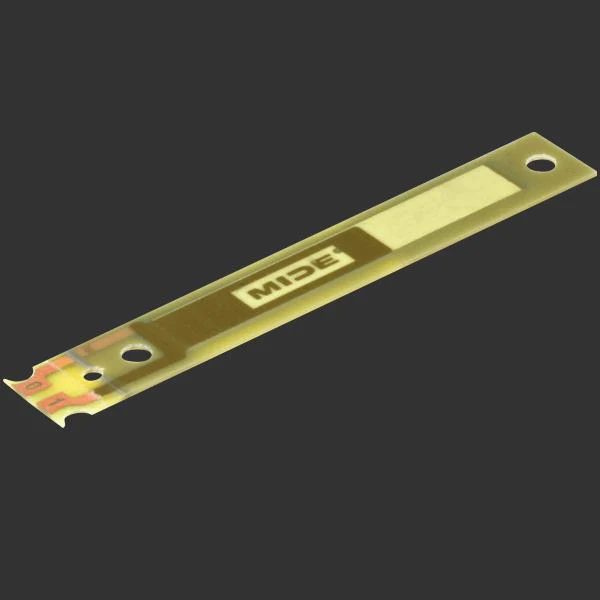
\includegraphics[scale=0.2]{img/peizo.png}
        \end{figure}

    \end{frame}

    \begin{frame}
        \frametitle{Resultaten Energy Harvesting}
        Pieken van 1.2 mW.
        \begin{figure}[h]
            \raggedright
            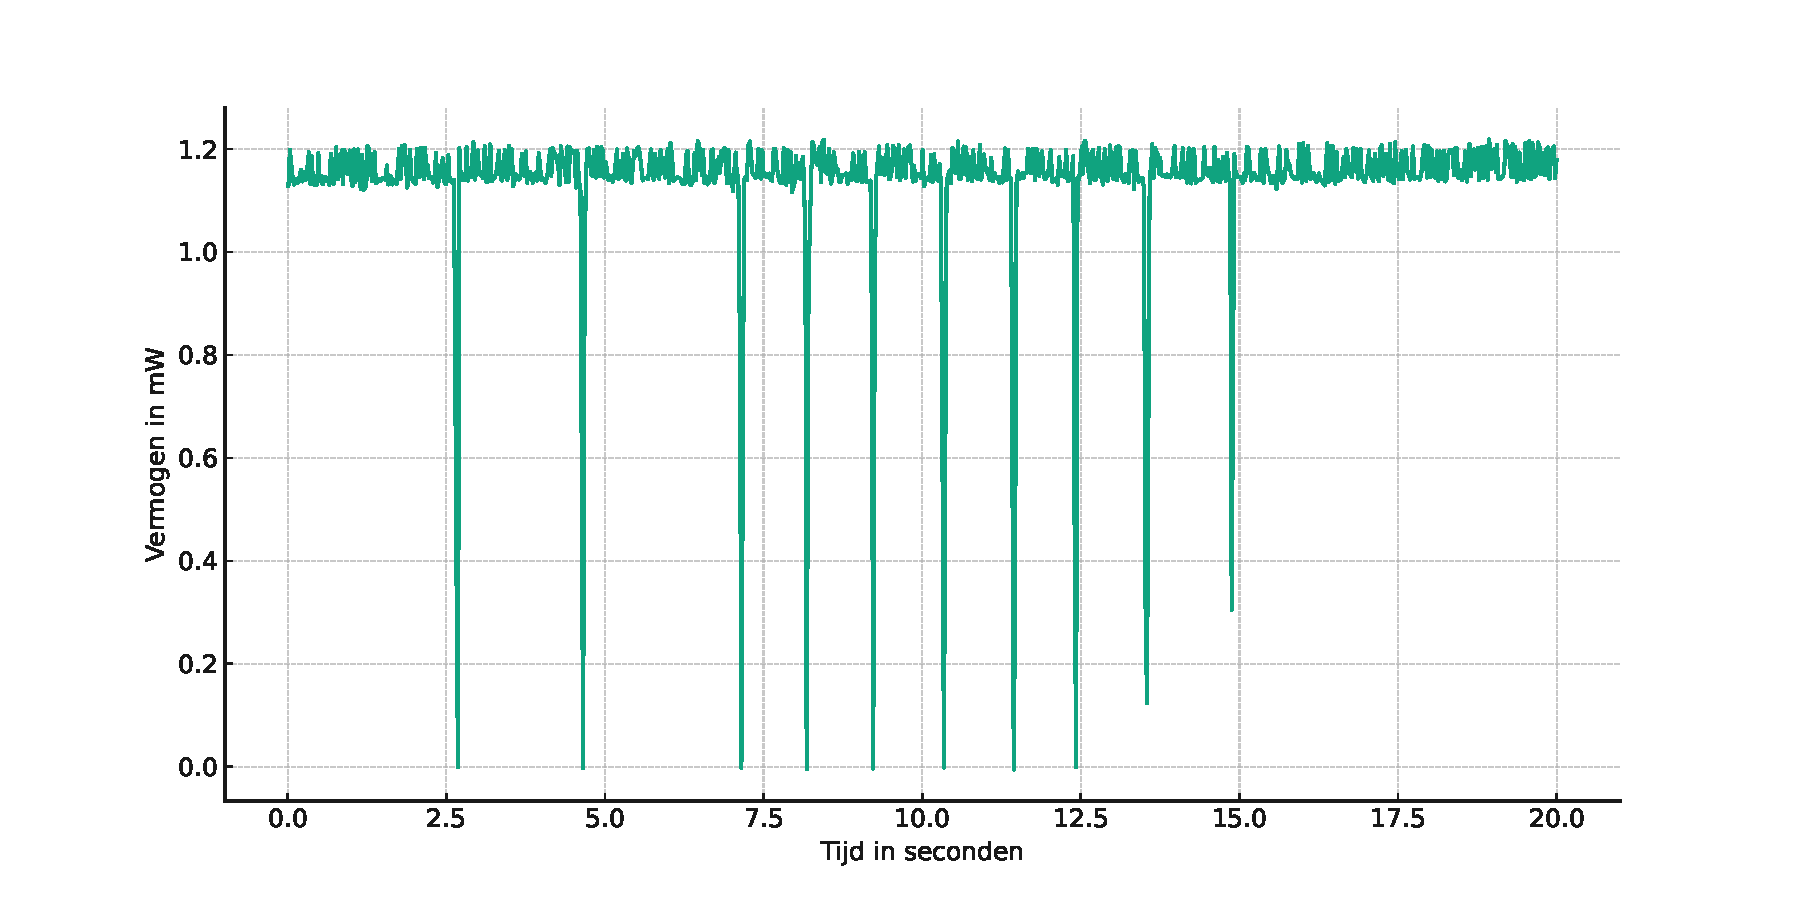
\includegraphics[scale=0.40]{img/resultaten_piezo.pdf}
        \end{figure}
    \end{frame}

    \subsection{Batterij}
    \begin{frame}
        \frametitle{Batterij}
        Gekozen voor Lithium-ion technologie
        \begin{itemize}
            \item Multicomp LIR2450
            \item 
            \begin{tabular}{|l|c c c|}
                \hline
                 & min & nom & max \\ \hline
                Spanning    & 2.7 V   & 3.6 V   & 4.2 V\\ \hline
                Capaciteit  & 110 mAh & 120 mAh &      \\ \hline
            \end{tabular}            
        \end{itemize}
        \begin{figure}[h]
            \raggedleft
            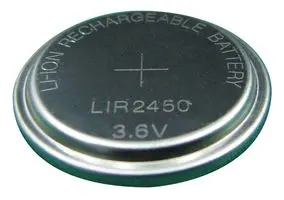
\includegraphics[scale=0.3]{img/batterij.png}
        \end{figure}
    \end{frame}
        

    \begin{frame}
        \frametitle{BMS}
        Eisen voor BMS
        \begin{itemize}
            \item Lage stroom verbruik
            \item Beveiligt voor:
                \begin{itemize}
                    \item Over laden
                    \item Over ontladen
                \end{itemize}
            \item Kan de stroom aan van het systeem
            
        \end{itemize}
        
        
    
    \end{frame}

    \begin{frame}
        \frametitle{LTC4071}
        \begin{itemize}
            \item 550 nA tijdens werking
            \item $<$0.1 nA na 'Low battery disconnect'
            \item Max spanning 4.2 V
            \item 'Low battery disconnect' instelbaar
                \begin{itemize}
                    \item 2.7 V Lithium Ion (Li-ion)
                    \item 3.2 V Lithium Polymeer (LiPo)
                \end{itemize}
            \item Bij overspanning, 50 mA shunt naar GND
            \item Stroom uitgang
                \begin{itemize}
                    \item $\pm 60$ mA continu 
                    \item 400 mA kleine pulse van $<$10ms
                \end{itemize}
        \end{itemize}

    \end{frame}

    \subsection{Spanning omzetting}

    \begin{frame}
        \frametitle{PMIC}
        \begin{figure}[h]
            \centering
            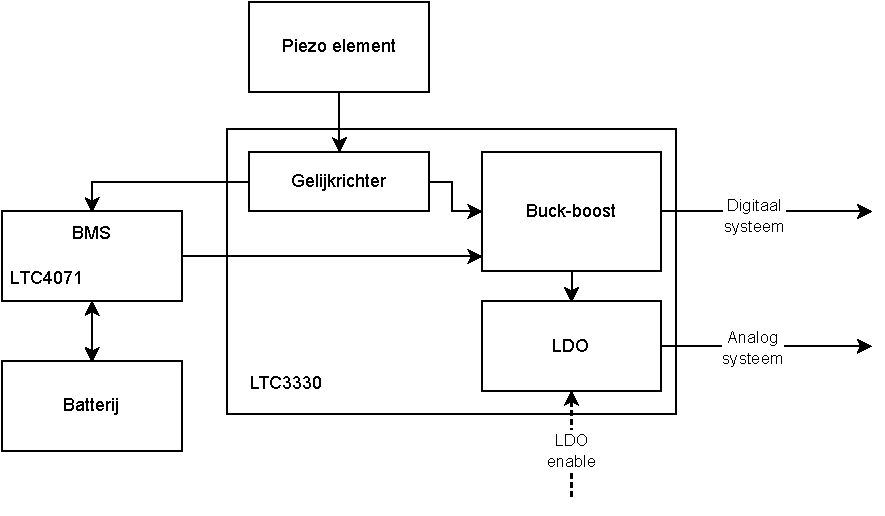
\includegraphics[scale=0.6]{img/energie_systeem.pdf}
        \end{figure}
    \end{frame}

    \begin{frame}
        \frametitle{Energieverbruik energie system}
        \begin{tabular}{|l|c|}
        \hline
            & Vermogen \\ \hline
            Buck-boost & 0.13 mW* \\ \hline
            Buck-boost + LDO  & 0.38 mW*\\ \hline
        \end{tabular} \\       
        *LTC4071 verbruik zit bij de metingen\\
        metingen gedaan zonder load.
        \vspace{1cm}

            \centering
            Uit specificaties max verbruik energiesysteem 1 mW.\\ 
            $0.38$ mW $< 1$ mW\\
            Dus energie deel voldoet aan max verbruik specificaties. 

    \end{frame}

    % \begin{frame}
    %     \frametitle{Demo}
    
        
    
    % \end{frame}